\documentclass[twocolumn]{article}
\usepackage[utf8]{inputenc}
\usepackage[top=1in]{geometry}
\usepackage{graphicx}
\usepackage{booktabs}
\usepackage{amsmath}
% Calligraphic fonts
\newcommand{\calA}{{\cal A}}
\newcommand{\calB}{{\cal B}}
\newcommand{\calC}{{\cal C}}
\newcommand{\calD}{{\cal D}}
\newcommand{\calE}{{\cal E}}
\newcommand{\calF}{{\cal F}}
\newcommand{\calG}{{\cal G}}
\newcommand{\calH}{{\cal H}}
\newcommand{\calI}{{\cal I}}
\newcommand{\calJ}{{\cal J}}
\newcommand{\calK}{{\cal K}}
\newcommand{\calL}{{\cal L}}
\newcommand{\calM}{{\cal M}}
\newcommand{\calN}{{\cal N}}
\newcommand{\calO}{{\cal O}}
\newcommand{\calP}{{\cal P}}
\newcommand{\calQ}{{\cal Q}}
\newcommand{\calR}{{\cal R}}
\newcommand{\calS}{{\cal S}}
\newcommand{\calT}{{\cal T}}
\newcommand{\calU}{{\cal U}}
\newcommand{\calV}{{\cal V}}
\newcommand{\calW}{{\cal W}}
\newcommand{\calX}{{\cal X}}
\newcommand{\calY}{{\cal Y}}
\newcommand{\calZ}{{\cal Z}}

% Sets:
\newcommand{\setA}{\textsf{A}}
\newcommand{\setB}{\textsf{B}}
\newcommand{\setC}{\textsf{C}}
\newcommand{\setD}{\textsf{D}}
\newcommand{\setE}{\textsf{E}}
\newcommand{\setF}{\textsf{F}}
\newcommand{\setG}{\textsf{G}}
\newcommand{\setH}{\textsf{H}}
\newcommand{\setI}{\textsf{I}}
\newcommand{\setJ}{\textsf{J}}
\newcommand{\setK}{\textsf{K}}
\newcommand{\setL}{\textsf{L}}
\newcommand{\setM}{\textsf{M}}
\newcommand{\setN}{\textsf{N}}
\newcommand{\setO}{\textsf{O}}
\newcommand{\setP}{\textsf{P}}
\newcommand{\setQ}{\textsf{Q}}
\newcommand{\setR}{\textsf{R}}
\newcommand{\setS}{\textsf{S}}
\newcommand{\setT}{\textsf{T}}
\newcommand{\setU}{\textsf{U}}
\newcommand{\setV}{\textsf{V}}
\newcommand{\setW}{\textsf{W}}
\newcommand{\setX}{\textsf{X}}
\newcommand{\setY}{\textsf{Y}}
\newcommand{\setZ}{\textsf{Z}}

% Vectors
\newcommand{\bfa}{\mathbf{a}}
\newcommand{\bfb}{\mathbf{b}}
\newcommand{\bfc}{\mathbf{c}}
\newcommand{\bfd}{\mathbf{d}}
\newcommand{\bfe}{\mathbf{e}}
\newcommand{\bff}{\mathbf{f}}
\newcommand{\bfg}{\mathbf{g}}
\newcommand{\bfh}{\mathbf{h}}
\newcommand{\bfi}{\mathbf{i}}
\newcommand{\bfj}{\mathbf{j}}
\newcommand{\bfk}{\mathbf{k}}
\newcommand{\bfl}{\mathbf{l}}
\newcommand{\bfm}{\mathbf{m}}
\newcommand{\bfn}{\mathbf{n}}
\newcommand{\bfo}{\mathbf{o}}
\newcommand{\bfp}{\mathbf{p}}
\newcommand{\bfq}{\mathbf{q}}
\newcommand{\bfr}{\mathbf{r}}
\newcommand{\bfs}{\mathbf{s}}
\newcommand{\bft}{\mathbf{t}}
\newcommand{\bfu}{\mathbf{u}}
\newcommand{\bfv}{\mathbf{v}}
\newcommand{\bfw}{\mathbf{w}}
\newcommand{\bfx}{\mathbf{x}}
\newcommand{\bfy}{\mathbf{y}}
\newcommand{\bfz}{\mathbf{z}}


\newcommand{\bfalpha}{\boldsymbol{\alpha}}
\newcommand{\bfbeta}{\boldsymbol{\beta}}
\newcommand{\bfgamma}{\boldsymbol{\gamma}}
\newcommand{\bfdelta}{\boldsymbol{\delta}}
\newcommand{\bfepsilon}{\boldsymbol{\epsilon}}
\newcommand{\bfzeta}{\boldsymbol{\zeta}}
\newcommand{\bfeta}{\boldsymbol{\eta}}
\newcommand{\bftheta}{\boldsymbol{\theta}}
\newcommand{\bfiota}{\boldsymbol{\iota}}
\newcommand{\bfkappa}{\boldsymbol{\kappa}}
\newcommand{\bflambda}{\boldsymbol{\lambda}}
\newcommand{\bfmu}{\boldsymbol{\mu}}
\newcommand{\bfnu}{\boldsymbol{\nu}}
\newcommand{\bfomicron}{\boldsymbol{\omicron}}
\newcommand{\bfpi}{\boldsymbol{\pi}}
\newcommand{\bfrho}{\boldsymbol{\rho}}
\newcommand{\bfsigma}{\boldsymbol{\sigma}}
\newcommand{\bftau}{\boldsymbol{\tau}}
\newcommand{\bfupsilon}{\boldsymbol{\upsilon}}
\newcommand{\bfphi}{\boldsymbol{\phi}}
\newcommand{\bfchi}{\boldsymbol{\chi}}
\newcommand{\bfpsi}{\boldsymbol{\psi}}
\newcommand{\bfomega}{\boldsymbol{\omega}}
\newcommand{\bfxi}{\boldsymbol{\xi}}
\newcommand{\bfell}{\boldsymbol{\ell}}

% Matrices
\newcommand{\bfA}{\mathbf{A}}
\newcommand{\bfB}{\mathbf{B}}
\newcommand{\bfC}{\mathbf{C}}
\newcommand{\bfD}{\mathbf{D}}
\newcommand{\bfE}{\mathbf{E}}
\newcommand{\bfF}{\mathbf{F}}
\newcommand{\bfG}{\mathbf{G}}
\newcommand{\bfH}{\mathbf{H}}
\newcommand{\bfI}{\mathbf{I}}
\newcommand{\bfJ}{\mathbf{J}}
\newcommand{\bfK}{\mathbf{K}}
\newcommand{\bfL}{\mathbf{L}}
\newcommand{\bfM}{\mathbf{M}}
\newcommand{\bfN}{\mathbf{N}}
\newcommand{\bfO}{\mathbf{O}}
\newcommand{\bfP}{\mathbf{P}}
\newcommand{\bfQ}{\mathbf{Q}}
\newcommand{\bfR}{\mathbf{R}}
\newcommand{\bfS}{\mathbf{S}}
\newcommand{\bfT}{\mathbf{T}}
\newcommand{\bfU}{\mathbf{U}}
\newcommand{\bfV}{\mathbf{V}}
\newcommand{\bfW}{\mathbf{W}}
\newcommand{\bfX}{\mathbf{X}}
\newcommand{\bfY}{\mathbf{Y}}
\newcommand{\bfZ}{\mathbf{Z}}


\newcommand{\bfGamma}{\boldsymbol{\Gamma}}
\newcommand{\bfDelta}{\boldsymbol{\Delta}}
\newcommand{\bfTheta}{\boldsymbol{\Theta}}
\newcommand{\bfLambda}{\boldsymbol{\Lambda}}
\newcommand{\bfPi}{\boldsymbol{\Pi}}
\newcommand{\bfSigma}{\boldsymbol{\Sigma}}
\newcommand{\bfUpsilon}{\boldsymbol{\Upsilon}}
\newcommand{\bfPhi}{\boldsymbol{\Phi}}
\newcommand{\bfPsi}{\boldsymbol{\Psi}}
\newcommand{\bfOmega}{\boldsymbol{\Omega}}


% Blackboard Bold:
\newcommand{\bbA}{\mathbb{A}}
\newcommand{\bbB}{\mathbb{B}}
\newcommand{\bbC}{\mathbb{C}}
\newcommand{\bbD}{\mathbb{D}}
\newcommand{\bbE}{\mathbb{E}}
\newcommand{\bbF}{\mathbb{F}}
\newcommand{\bbG}{\mathbb{G}}
\newcommand{\bbH}{\mathbb{H}}
\newcommand{\bbI}{\mathbb{I}}
\newcommand{\bbJ}{\mathbb{J}}
\newcommand{\bbK}{\mathbb{K}}
\newcommand{\bbL}{\mathbb{L}}
\newcommand{\bbM}{\mathbb{M}}
\newcommand{\bbN}{\mathbb{N}}
\newcommand{\bbO}{\mathbb{O}}
\newcommand{\bbP}{\mathbb{P}}
\newcommand{\bbQ}{\mathbb{Q}}
\newcommand{\bbR}{\mathbb{R}}
\newcommand{\bbS}{\mathbb{S}}
\newcommand{\bbT}{\mathbb{T}}
\newcommand{\bbU}{\mathbb{U}}
\newcommand{\bbV}{\mathbb{V}}
\newcommand{\bbW}{\mathbb{W}}
\newcommand{\bbX}{\mathbb{X}}
\newcommand{\bbY}{\mathbb{Y}}
\newcommand{\bbZ}{\mathbb{Z}}




\title{Homework 6}
\author{Max marks: 50 marks}
\date{Due on Oct 25th, 2021, 9 AM, before class.}
\newtheorem{prob}{Problem}

\newcommand{\bw}{\bar{w}}
\newcommand{\bx}{\bar{x}}
\newcommand{\by}{\bar{y}}
\newcommand{\bz}{\bar{z}}
\newcommand{\bA}{\bar{A}}
\newcommand{\bB}{\bar{B}}
\newcommand{\bC}{\bar{C}}
\begin{document}

\maketitle
\begin{prob}
  Show how the function $f (w_1 , w_2 , w_3 ) = \sum m(0, 2, 3, 4, 5, 7)$ can be implemented using a
  3-to-8 binary decoder and an OR gate.~\cite[Prob 4.1]{brown2013fundamentals}
  (10 marks)
\end{prob}

\begin{prob}
  Consider the function $f = \bw_2 \bw_3 + w_1 w_2$.  Derive a circuit for
  $f$ that uses only one 2-to-1 multiplexer and no other gates (assuming inputs
  are available in both uncomplemented and complemented form).~\cite[Prob 4.4]{brown2013fundamentals}(10 marks)
\end{prob}

\begin{prob}
  Figure~\ref{fig:seven-seg-display} shows the notation for a BCD to 7-segment
display and Table~\ref{tab:seven-segment-tt} shows the corresponding truth
table. The inputs corresponding to the missing rows in the truth table should be
considered as don't care.
  \begin{enumerate}
   \item implement segment ``a'' using an 8:1 mux and no other logic gate, (10 marks)
   \item implement segment ``a'' using a 4:1 mux and one other gate, (10 marks)
   \item implement segment ``f'' with 4:1 mux and no other logic gate. Assume
     inputs are available in both uncomplemented and complemented form. (Hint:
     There are (${}^4C_2 = 6$) possible pairs of control inputs: ($w_3, w_2$), ($w_2, w_1$),
     ($w_1,w_0$), ($w_0, w_3$), ($w_0, w_2$), ($w_1, w_3$). There are 6 don't
     care conditions. With two control inputs of the multiplexer and one input
     allowed, you can represent an expression with upto 4-SOP-terms of size
     three-literals or less.) (10 marks)
  \end{enumerate}
\end{prob}

\begin{figure}[h]
  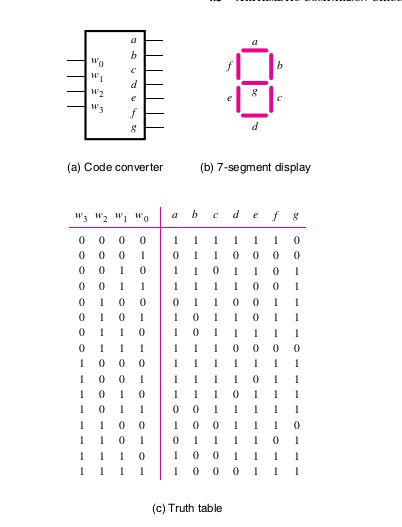
\includegraphics[width=\linewidth,trim=0 10cm 0 0.2cm,clip]{fig-4.21.png}
  \\
  \caption{Seven segment display and BCD-to-7-segment display converter. When
    $a=1$ the corresponding segment of the display lights up. To display the
    number 8, you will turn on all the seven segments, while to display 1, you
    will turn on $b=1, c=1$ and turn off $=0$ the rest. The full truth-table for
  the seven-segment display is shown in Table~\ref{tab:seven-segment-tt}.}
  \label{fig:seven-seg-display}
\end{figure}

\begin{table}
  \footnotesize
\begin{tabular}{l|cccc||ccccccc}
  \toprule
  Row & $w_3$ & $w_2$ & $w_1$ & $w_0$ & a & b & c & d & e & f & g \\
  \midrule
  0  & 0    & 0   &   0 &   0 & 1 & 1 & 1 & 1 & 1 & 1 & 0 \\
  1  & 0    & 0   &   0 &   1 & 0 & 1 & 1 & 0 & 0 & 0 & 0 \\
  2  & 0    & 0   &   1 &   0 & 1 & 1 & 0 & 1 & 1 & 0 & 1 \\ 
  3  & 0    & 0   &   1 &   1 & 1 & 1 & 1 & 1 & 0 & 0 & 1 \\ 
  4  & 0    & 1   &   0 &   0 & 0 & 1 & 1 & 0 & 0 & 1 & 1 \\ 
  5  & 0    & 1   &   0 &   1 & 1 & 0 & 1 & 1 & 0 & 1 & 1 \\   
  6  & 0    & 1   &   1 &   0 & 1 & 0 & 1 & 1 & 1 & 1 & 1 \\ 
  7  & 0    & 1   &   1 &   1 & 1 & 1 & 1 & 0 & 0 & 0 & 0 \\ 
  8  & 1    & 0   &   0 &   0 & 1 & 1 & 1 & 1 & 1 & 1 & 1 \\
  9  & 1    & 0   &   0 &   1 & 1 & 1 & 1 & 1 & 0 & 1 & 1 \\
  \bottomrule
\end{tabular}
\caption{Truth table for BCD to seven-segment display as shown in
  Figure~\ref{fig:seven-seg-display}. The missing combinations of inputs should
  be considered as dont care.}
\label{tab:seven-segment-tt}
\end{table}

\bibliography{main}
\bibliographystyle{plain}
\end{document}
